\chapter{Introduzione}
\label{cha:intro}

Le sospensioni semi-attive sono costituite da ammortizzatori a smorzamento variabile e sono realizzate in modo tale che non sia possibile somministrare ulteriore energia meccanica al sistema, a differenza delle sospensione attive che sono costituite da attuatori che esercitano  una forza indipendente.\\
Le sospensioni semi-attive offrono affidabilità e prestazioni migliori rispetto alle sospensioni passive, mantenendo allo stesso tempo l'efficienza e l'ottima versatilità dei sistemi attivi, senza però aver bisogno di fonti di energia, rendendo possibile un risparmio dal punto di vista economico.\\

Il tipo di sospensione semi-attiva preso in esame in questa tesi è quello costituito da ammortizzatori che sfruttano gli effetti magnetoreologici di alcuni fluidi, come l'olio. La peculiarità di questi fluidi è che possono variare la propria viscosità in base all'azione di campi magnetici esterni, la cui intensità può essere facilmente regolata da un semplice circuito elettromagnetico. In questo modo è possibile modificare la forza di smorzamento esercitata dalla sospensione, senza cambiare la sua geometria. Controllare questo tipo di sospensione è un compito non banale, in quanto anche nella configurazione passiva, cioè quando l'ingresso di controllo è mantenuto costante, la sospensione magnetoreologica fornisce un comportamento non lineare.\\

\section{Modello quarter car}
L'analisi del comportamento dinamico di un veicolo può rivelarsi molto complessa, per questo si utilizzano dei modelli semplificati. Uno dei principali è il modello quarter car che descrive la dinamica verticale di un quarto dell'intero veicolo, concentrando l'analisi su una singola ruota e sul relativo sistema di sospensioni, trascurando le interazioni tra le varie parti del veicolo. Questo tipo di modello, rappresentato in \figurename \  \ref{fig:quarter-car}, è caratterizzato da una massa sospesa \textit{$m_s$}, corrispondente a un quarto della massa del telaio del veicolo e da una massa non sospesa \textit{$m_u$} che rappresenta la ruota. Queste due sono connesse dalla sospensione, modellata da una molla elastica di costante \textit{k} e dall'elemento \textit{$f_d$} che rappresenta lo smorzatore magnetoreologico. Inoltre, la molla elastica \textit{$k_t$}, posta tra massa non sospesa e profilo stradale, descrive la rigidezza della ruota.
\begin{figure}[hbt]
	\centering
	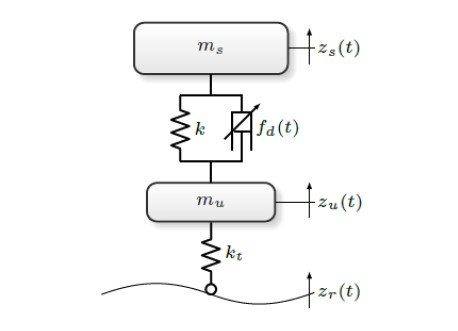
\includegraphics[scale=0.8]{figure/modello-quarter-car.jpg}
	\caption{Rappresentazione schematica del modello quarter car}
	\label{fig:quarter-car}
\end{figure}\\
Il modello matematico che descrive lo schema rappresentato in \figurename \ \ref{fig:quarter-car} può essere ottenuto considerando la legge di Newton per ognuna delle due masse, \textit{$m_s$} e \textit{$m_u$}, che si muovono lungo l'asse verticale. Le equazioni differenziali sono dunque le seguenti:
\begin{equation}
	\centering
	\begin{cases}
		m_s\ddot{z}_s = -k\tilde{z} - f_d(\dot{\tilde{z}})\\
		m_s\ddot{z}_u = -k_t(z_u - z_r) + k\tilde{z} + f_d(\dot{\tilde{z}}),\\
	\end{cases}
	\label{eqprinc}
\end{equation}\\
dove $\ddot{z}_s$, $\dot{z}_s$ e $z_s$ sono rispettivamente l'accelerazione, la velocità e lo spostamento della massa $m_s$ e $\ddot{z}_u$, $\dot{z}_u$ e $z_u$ sono l'accelerazione, la velocità e lo spostamento della massa $m_u$. Mentre $\tilde{z} := z_s - z_u$, $\dot{\tilde{z}}$ è la velocità di avanzamento e $z_r$ rappresenta il profilo stradale. Come detto pocanzi, \textit{$f_d$} è il termine che descrive la forza di smorzamento che introduce una forte non-linearità nel sistema.\\

Per lo svolgimento della tesi sono stati considerati valori numerici assimilabili a quelli di un SUV. Nella \tablename \ \ref{parametri} sono elencati i parametri del modello quarter car e della sospensione magnetoreologica.

\renewcommand\arraystretch{1.4} 
\begin{table}[hbt]
	\centering
	\begin{tabular}{|c||c|c|}
		\hline
		\textbf{Parametro} & \textbf{Simbolo} & \textbf{Valore} \\
		\hline	Massa della Ruota & \textit{$m_u$} & 70 \textit{Kg}\\
		\hline	Massa di $\frac{1}{4}$ di Veicolo & \textit{$m_s$} & 450 \textit{Kg}\\
		\hline	Rigidezza Sospensione & \textit{$k$} & 27000 \textit{$\frac{N}{M}$}\\
		\hline	Rigidezza Ruota & \textit{$k_t$} & 300000 \textit{$\frac{N}{M}$}\\
		\hline	Smorzamento minimo & \textit{$c_{min}$} & 800 \textit{$\frac{N s}{M}$}\\
		\hline	Pendenza di saturazione & \textit{$k_0$} & 38000 \textit{$\frac{N s}{M}$}\\
		\hline	Livello massimo di saturazione & \textit{$\tilde{f}_{max}$} & 3000 \textit{N}\\		
		\hline
	\end{tabular}
	\caption{Parametri modello quarter car e sospensione MR}
	\label{parametri}
\end{table}


\section{Implementazione modello in MATLAB \& Simulink}
Il passo successivo è stato quello di implementare in Simulink il modello quarter car del veicolo, secondo il sistema di equazioni \ref{eqprinc}. Con l'utilizzo di MATLAB sono stati definiti tutti i parametri utili, sono state lanciate tutte le simulazioni e sono stati raccolti tutti i risultati.\\
\begin{figure}[hbt]
	\centering
	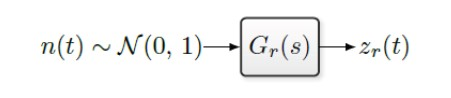
\includegraphics[scale=0.5]{figure/zr.jpg}
	\caption{Schema generazione profilo stradale}
	\label{fig:zr}
\end{figure}\\
La variazione del profilo stradale rappresenta l'input esterno del sistema ed è stato calcolato, come mostra la \figurename \ \ref{fig:zr}, filtrando un rumore gaussiano $n(t)$, attraverso la funzione di trasferimento $G_r(t)$ \eqref{Gr}. Questo tipo di approccio, utilizzato da \cite{controlMRdampers}, per definire il profilo stradale, è un'implementazione equivalente alla generazione di un profilo stradale secondo la normativa ISO-8608.
\begin{equation}
	\centering
	G_r(s) = \frac{s}{s^2 + 2\xi_r\omega_rs + \omega_r^2}
	\label{Gr}
\end{equation}
dove $\xi_r = 0.7$ e $\omega_r$ dipende dalla velocità del veicolo secondo la formula:
\begin{equation}
	\centering
	\omega_r = \frac{2\pi v}{l_c}
	.
	\label{omega_r}
\end{equation}
Il parametro $l_c$ è costante e rappresenta la massima risoluzione spaziale considerata, dove un valore piccolo del parametro corrisponde a considerare una strada quasi piatta con delle micro-asperità distribuite. La velocità considerata per tutte le simulazioni è pari a $v = 90\frac{km}{h}$.\\
In \figurename \ \ref{fig:profilostradale} è mostrato un esempio del profilo stradale ottenuto in MATLAB.
\begin{figure}[hbt]
	\centering
	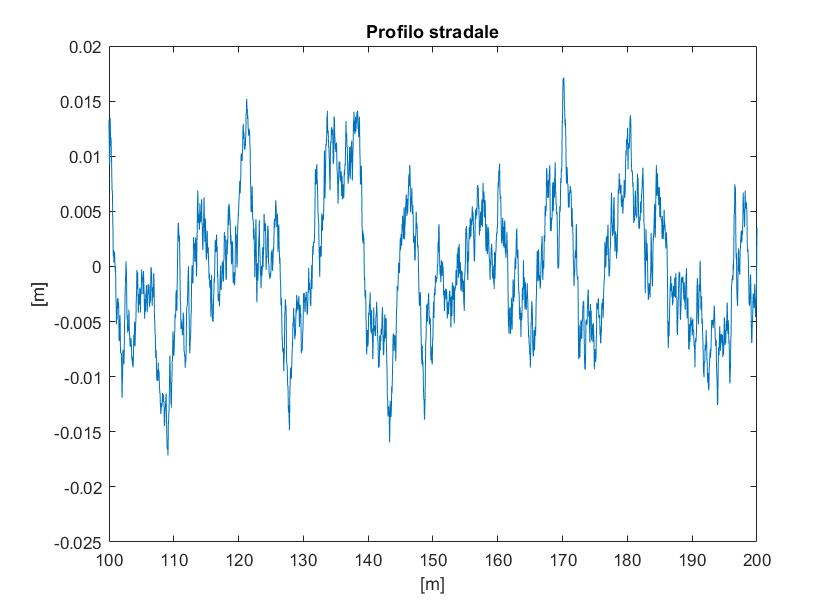
\includegraphics[scale=0.3]{figure/profilostradale.jpg}
	\caption{Esempio grafico profilo stradale}
	\label{fig:profilostradale}
\end{figure}\\
Il profilo stradale viene generato a seguito di un processo casuale, quindi i risultati possono variare da una simulazione all'altra. Per evitare una variabilità troppo alta, è stata considerato un tratto di strada sufficentemente lungo, di 2.5$km$.\\

Riepilogando, il sistema dinamico ha come ingresso la variazione del profilo stradale $z_r$, il vettore delle variabili di stato è definito come $x = [\dot{z_s}\ z_s\ \dot{\tilde{z}}\ \tilde{z}]^T $, mentre l'uscita corrisponde all'accelerazione verticale $\ddot{z_s}$ di $\frac{1}{4}$ del veicolo.\\
Il termine $f_d(\dot{\tilde{z}})$ che descrive la relazione di non-linearità tra forza dello smorzatore MR e velocità di avanzamento, presente in \eqref{eqprinc}, è definito dalla seguente equazione:
\begin{equation}
	\centering
	f_d = c_{min}*(\dot{z_s}-\dot{z_u}) + \tilde{f_d}(u_{MR},\dot{z_s}-\dot{z_u})
	.
	\label{fd}
\end{equation}
L'equazione \eqref{fd} è composta da un termine lineare, il quale rappresenta il minimo smorzamento, e dal termine $\tilde{f_d}$ che descrive la nonlinearità della sospensione ed è definito come:
\begin{equation}
	\centering
	\tilde{f_d}(u_{MR},\dot{z_s}-\dot{z_u}) = sat_{u_{MR}}(k_0(\dot{z_s} - \dot{z_u}))
	,
	\qquad\qquad u_{MR} \epsilon [0,\tilde{f}_{max}]
	\label{fdtilde}
\end{equation}
\'E importante notare come nell'equazione \eqref{fdtilde}, la variabile di controllo $u_{MR}$ della sospensione semi-attiva è definita in modo esplicito e corrisponde ai limiti della saturazione.\\	

Le prime simulazioni, fatte per familiarizzare meglio con il simulatore, sono state svolte con una configurazione passiva, cioè quando l'ingresso di controllo è mantenuto costante per tutta la durata della simulazione, e solo in un secondo momento è stata implementata la legge di controllo.

\section{Indice di performance \textit{J}}
\begin{figure}[htb]
	\centering
	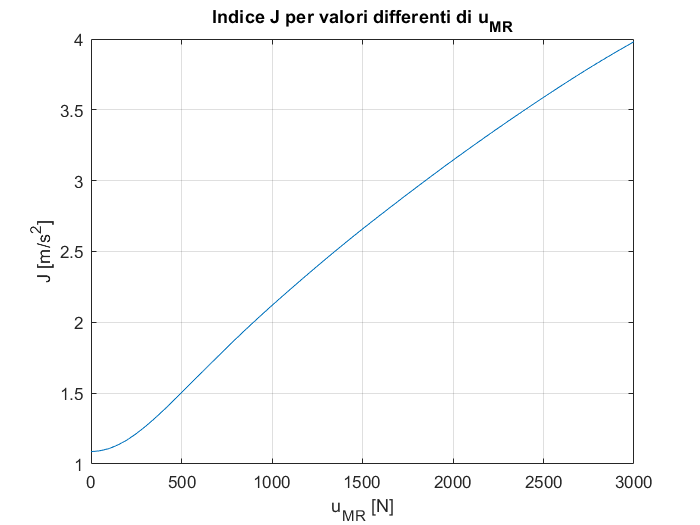
\includegraphics[scale=0.5]{figure/indice_performance.png}
	\caption{Indice di comfort per valori costanti differenti della variabile di controllo $u\textsubscript{MR} \epsilon [0,\tilde{f}_{max}]$}
	\label{fig:indiceperformance}
\end{figure}
Ci sono diversi modi per analizzare i dati di una simulazione e trarre delle conclusioni significative. Nel corso di questo lavoro è stata fatta particolare attenzione al valore dell'indice di performance, che corrisponde al valore dell'output del sistema $y = \ddot{z}_s$, come mostrato nell'equazione \eqref{indiceJ}.\\
Il confronto base per ogni strategia di controllo semi-attiva è la sospensione con una configurazione passiva e in questo caso è stato fatto in termini di comfort del passaggero, grazie all'indice \textit{J}.
\begin{equation}
	\centering
	J(\ddot{z}_s) = \left(\frac{1}{T}\int_{0}^{T}\lvert \ddot{z}_s(\tau) \rvert ^2 d\tau\right)^\frac{1}{2}
	\label{indiceJ}
\end{equation}
In \figurename \ \ref{fig:indiceperformance} è possibile visualizzare meglio l'andamento dell'indice \textit{J} in funzione di diversi valori della variabile di controllo $u_{MR}$. Si può notare come le prestazioni migliori, ${J\approx1.1\frac{m}{s^2}}$, siano ottenute con $u_{MR}\approx0$.


\section{Validazione del modello}
Per essere certi di aver fatto tutto correttamente, è stato necessario validare il modello implementato in Simulink con dei controesempi. In un primo momento sono state analizzate le simulazioni lineari, con $u_{MR}=0$, che risultano essere più semplici da verificare. Infatti, se $u_{MR} = 0$, il termine $\tilde{f}_d$ nell'equazione \eqref{fd} si annulla e quindi il modello non lineare si trasforma in uno lineare. Il blocco \textit{Space-State} di Simulink permette di implementare in modo semplice un sistema dinamico lineare: è sufficiente indicare le quattro matrici A, B, C e D che lo caratterizzano e l'input del sistema.  
\begin{equation}
	\centering
	\begin{cases}
		\dot{x} = Ax + Bz_r\\
		y = \ddot{z}_s = Cx + Dz_r\\
	\end{cases}
	\label{sistlineare}
\end{equation}

\begin{equation}
	\left[
	\begin{array}{c|c}
		A & B\\
		\hline
		C & D\\
	\end{array}
	\right] = \left[
	\begin{array}{c c c c|c}
		0 & 0 & 1 & 0 & 0\\
		0 & 0 & 0 & 1 & 0\\
		0 & -\frac{k}{m_s} & 0 & -\frac{c_{min}}{m_s} & 0\\
		\frac{k_t}{m_u} & -\frac{k}{m_s}-\frac{k_t + k}{m_u} & 0 & -\frac{c_{min}(m_s + m_u)}{m_um_s} & -\frac{k_t}{m_u}\\
		\hline
		0 & -\frac{k}{m_s} & 0 & 0 & 0\\
	\end{array}
	\right]
\end{equation}

A questo punto è stato confrontato l'output $\ddot{z}_s$ dei due sistemi, tramite il blocco \textit{Scope} che mostra l'andamento dei segnali in funzione del tempo della simulazione. L'accelerazione si è rivelata essere identica per entrambi i modelli, risultato che conferma la validità del simulatore realizzato.\\
Un' ulteriore analisi è stata fatta nel dominio della frequenza, dove è stata verificata l'uguaglianza delle funzioni di trasferimento dei due modelli. Per entrambi i sistemi è stata utilizzata la funzione \textit{tfestimate} di Matlab e come si evince dalla \figurename \ \ref{fig:Fdtconfronto}, i due grafici sono risultati essere perfettamente uguali.
\begin{figure}[hbt]
	\centering
	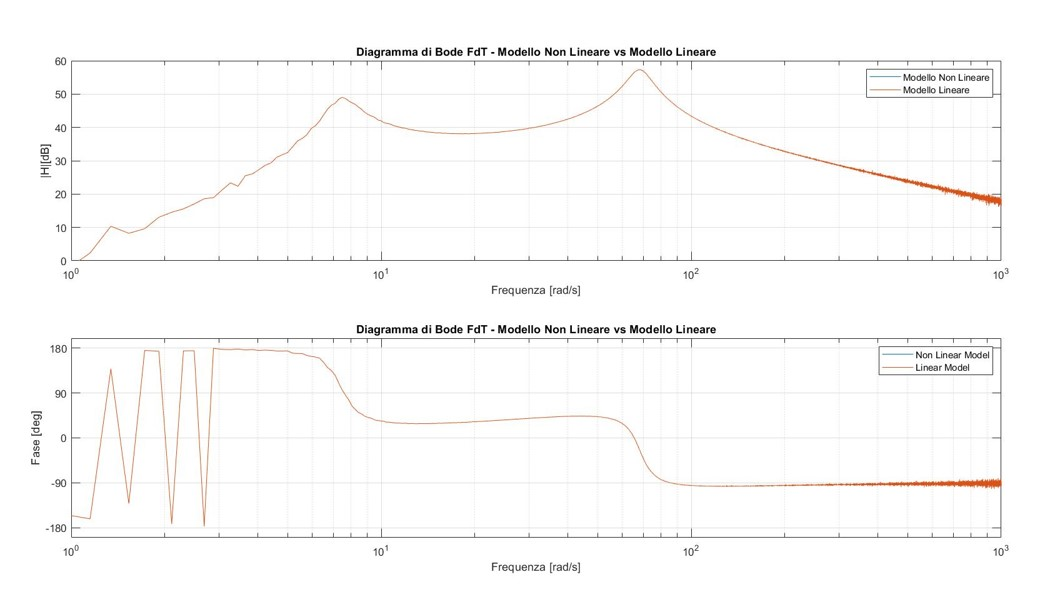
\includegraphics[scale=0.7]{figure/FdTconfronto.jpg}
	\caption{Confronto Funzione di Trasferimento modello lineare e non lineare}
	\label{fig:Fdtconfronto}
\end{figure}

Per quanto riguarda le simulazioni "non-lineari", con $u_{MR}\neq0$, è stato fatto un grafico della forza della sospensione in funzione della velocità di stroke $\dot{z}_s - \dot{z}_u$ e si è verificata l'uguaglianza con le mappe attese, vedi \cite{controlMRdampers}.
\begin{figure}[hbt]
	\centering
	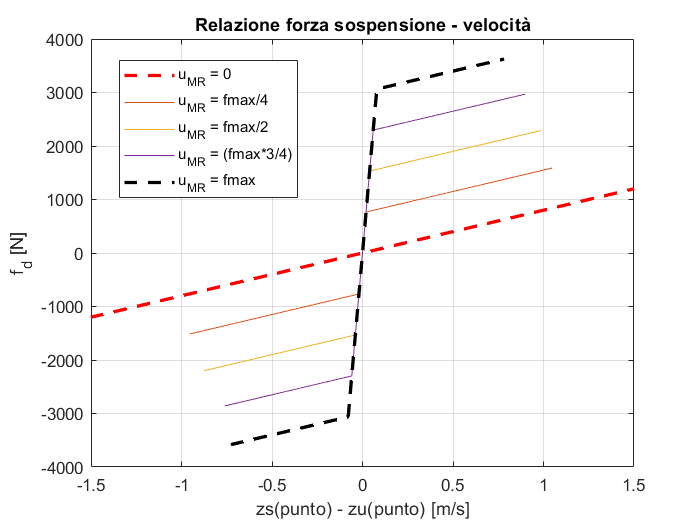
\includegraphics[scale=0.45]{figure/force-speed graph.png}
	\caption{Relazione tra forza e velocità della sospensione MR, con diveri valori di $u_{MR}$}
	\label{fig:graficofd}
\end{figure}

\section{Legge di controllo}
Una volta che il modello in Simulink è stato verificato ed è risultato corretto, il passo successivo e fondamentale per lo svolgimento della tesi è stato quello di implementare la legge di controllo.\\
In questo lavoro il controllore progettato per il sistema è un tipo di retroazione di stato standard, ottenuto a seguito di alcune manipolazioni, necessarie per poter essere applicato alla dinamica delle sospensioni MR, come mostrato in \cite{controlMRdampers}.\\
Nel corso di questa tesi sono state analizzate inizialmente le prestazioni di due diverse leggi di controllo, una di tipo lineare \eqref{leggelin} e una quadratica \eqref{leggequad}. A seguito però dei risultati ottenuti nel caso lineare e in quello quadratico, che saranno presentati successivamente, si è voluto implementare un'ulteriore legge di controllo, ottenuta sommando il termine lineare con quello quadratico \eqref{leggelinquad}. Le rispettive equazioni della variabile di controllo $u_{MR}$, che generano l'effettiva forza $\tilde{f}_d$ della sospensione, risultano essere:
\begin{equation}
	\centering
	u_{MR} = \frac{\tilde{f}_{max}}{2} + sgn(\dot{\tilde{z}})sat_{\frac{\tilde{f}_{max}}{2}}(\tilde{k}x),
	\label{leggelin}
\end{equation}
\begin{equation}
	\centering
	u_{MR} = \frac{\tilde{f}_{max}}{2} + sgn(\dot{\tilde{z}})sat_{\frac{\tilde{f}_{max}}{2}}(xP_xx^T),
	\label{leggequad}
\end{equation}
\begin{equation}
	\centering
	u_{MR} = \frac{\tilde{f}_{max}}{2} + sgn(\dot{\tilde{z}})sat_{\frac{\tilde{f}_{max}}{2}}(\tilde{k}x + xP_xx^T).
	\label{leggelinquad}
\end{equation}
I termini $\tilde{k}$ e $P_x$ sono rispettivamente un vettore e una matrice simmetrica, rappresentano un guadagno di stato retroazionato, lineare e non lineare, e il valore degli elementi che li compongono sono stati calcolati tramite un algoritmo di ottimizzazione.\begin{equation*}
	\tilde{k} = [k_1 \ k_2 \ k_3 \ k_4]^T \ \ \ \ \ \ \ \
	P_x = 
	\begin{bmatrix}
		p_{1,1} & p_{1,2} & p_{1,3} & p_{1,4} \\
		p_{2,1} & p_{2,2} & p_{2,3} & p_{2,4} \\
		p_{3,1} & p_{3,2} & p_{3,3} & p_{3,4} \\
		p_{4,1} & p_{4,2} & p_{4,3} & p_{4,4}
	\end{bmatrix}
\end{equation*}
















